\documentclass[12pt]{report}
\usepackage[utf8]{inputenc}
\usepackage[T1]{fontenc}
\usepackage[margin=1in]{geometry}
\usepackage{listings}
\usepackage{xcolor}
\usepackage[most]{tcolorbox}
\usepackage{fontawesome5}
\usepackage{titlesec}
\usepackage{fancyhdr}
\usepackage{float}
\usepackage{tikz}
\usepackage{amsmath}
\usepackage{hyperref}
% Minimalistic Fonts
\usepackage[sfdefault]{inter} % Clean sans-serif for headings
    % Clean, modern serif for body text

\titleformat{\chapter}[display]
{\normalfont\huge\bfseries\color{black}} % Style of the text
{\filleft\color{red!60!black}\MakeUppercase{\chaptername} \Huge\thechapter} % "Chapter 1" alignment
{1ex}
{\titlerule\vspace{1ex}\filright} % A horizontal line under the title
[\vspace{1ex}\titlerule]

\title{Project HLM (QML)}
\author{Ajmain Adil Tahmid}
\date{2026-27}

\definecolor{navy}{RGB}{27, 33, 26}

\hypersetup{
	colorlinks=true,
	linkcolor=navy,
	filecolor=magenta,
	urlcolor=cyan,
}

% Define the Fun Fact Box Style
\newtcolorbox{funfactbox}[1]{
	colback=yellow!10!white,    % Background color
	colframe=orange!70!black,  % Border color
	fonttitle=\bfseries,       % Title font style
	title={\faLightbulb \hspace{0.5em} Fun Fact: #1}, % Title with icon
	enhanced,                  % Enable advanced features
	attach boxed title to top left={yshift=-2mm, xshift=2mm},
	boxed title style={colback=orange!70!black},
	drop shadow,                % Add a subtle shadow
	top=10pt,
	bottom=10pt,
	left=10pt,
	right=10pt,
	before skip=10pt,
	after skip=10pt
}

% Define specific colors and environments
\newtcolorbox{todobox}{
	colback=red!5!white,
	colframe=red!75!black,
	title=To-Do,
	enhanced,
	rounded corners,
	sharp corners=southwest,
	sharp corners=northwest,
	attach boxed title to top left={yshift=-1.8mm, xshift=3mm},
	boxed title style={colback=blue!40!white},
	boxrule=0px,
	leftrule=3px,
	top=10pt,
	bottom=10pt,
	left=10pt,
	right=10pt,
	before skip=10pt,
	after skip=10pt
}

\newtcolorbox{tipbox}{
	colback=green!5!white,
	colframe=green!50!black,
	title=Tip,
	enhanced,
	rounded corners,
	sharp corners=southwest,
	sharp corners=northwest,
	attach boxed title to top left={yshift=-1.8mm, xshift=3mm},
	boxed title style={colback=blue!40!white},
	boxrule=0px,
	leftrule=3px,
	top=10pt,
	bottom=10pt,
	left=10pt,
	right=10pt,
	before skip=10pt,
	after skip=10pt
}

\newtcolorbox{warningbox}{
	colback=orange!5!white,
	colframe=orange!80!black,
	title={\faQuestionCircle \hspace{0.5em} Warning},
	enhanced,
	rounded corners,
	sharp corners=southwest,
	sharp corners=northwest,
	attach boxed title to top left={yshift=-1.8mm, xshift=3mm},
	boxed title style={colback=blue!40!white},
	boxrule=0px,
	leftrule=3px,
	top=10pt,
	bottom=10pt,
	left=10pt,
	right=10pt,
	before skip=10pt,
	after skip=10pt
}

\newtcolorbox{notebox}{
	colback=blue!7!white,
	colframe=blue!70!black,
	fonttitle=\bfseries,
	title={\faQuestionCircle \hspace{0.5em} Note},
	enhanced,
	rounded corners,
	attach boxed title to top left={yshift=-2mm, xshift=2mm},
	boxed title style={colback=blue!70!black},
	top=10pt,
	bottom=10pt,
	left=10pt,
	right=10pt,
	before skip=10pt,
	after skip=10pt
}

% Simple command for quick usage
\newcommand{\funfact}[2]{\begin{funfactbox}{#1} #2 \end{funfactbox}}


\fancyhf{}
\fancyhead[L]{Project HLM}
\fancyhead[R]{\leftmark}
\fancyfoot[C]{\thepage}
\renewcommand{\headrulewidth}{0.4pt} % Thin line at the top
\pagestyle{fancy}


\begin{document}
	
	\maketitle
	
	\pagenumbering{Roman}
	\begin{abstract}
		\begin{center}
			A project to build the Quad Model Language
		\end{center}
	\end{abstract}
	
	\newpage
	
	\tableofcontents
	
	\newpage
	
	\pagenumbering{arabic}
	\chapter{Introduction}
	\label{sec:intro}
	\section{What is Project HLM?}
	\textbf{Project HLM} is a project focused on enhancing skills. Its main goal is to create a custom compiled programming language called \textbf{QML}.
	
	\vspace{1.5em}
	
	
	% Usage 1: Using the command
	%\funfact{The Eiffel Tower}{The Eiffel Tower can be 15 cm taller during the summer due to thermal expansion of the iron.}
	
	% Usage 2: Using the environment for longer facts
	\begin{funfactbox}{Naming of Project HLM}
		The “HLM” part is completely meaningless. Originally, I took inspiration from Helium ($^4_2H$)  (HLM → Helium), so I chose .hlm as the file extension, and now I’m just too lazy to rename it.
	\end{funfactbox}
	
	\vspace{0.5em}
	
	\section{What is QML?}
	QML is an abbreviation for \textit{Quad Model Language}. It is a programming language designed around a four-dimensional design model that captures the core trade-offs present in real-world language and system design.
	
	\vspace{1.5em}
	
	The fundamental structure of QML is the \textit{quad model}, which defines four primary design goals: \textbf{Power}, \textbf{Flexibility}, \textbf{Connectivity}, and \textbf{Precision}. These goals are intentionally placed in tension with one another, reflecting the reality that no programming language can maximize all dimensions simultaneously without compromise. QML is an exploration of control, responsibility, and trade-offs in low-level language design.
	
	\begin{figure}[H]
		\centering
		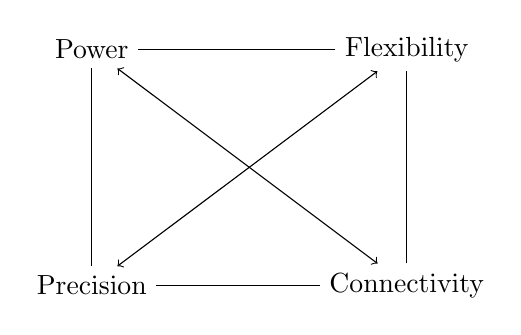
\begin{tikzpicture}
			\node (a) at (0.5,3.5) {Power};
			\node (b) at (4.5,3.5) {Flexibility};
			\node (c) at (4.5,0.5) {Connectivity};
			\node (d) at (0.5,0.5) {Precision};
			\draw (c) -- (b) -- (a) -- (d) -- (c);
			\draw[<->] (d) -- (b);
			\draw[<->] (c) -- (a);
		\end{tikzpicture}
		\caption{The primary quad model illustrating the four core design goals of QML.}
		\label{fig:mainquad}
	\end{figure}
	
	Figure~\ref{fig:mainquad} illustrates the primary quad model of QML and the relationships between these four goals. Each axis represents a dimension in which a language implementation may prioritize certain features over others. Rather than attempting to hide these trade-offs, QML exposes them explicitly as part of its design philosophy.
	
	As a result, QML encourages deliberate and transparent design decisions, allowing developers to reason clearly about the strengths and limitations of their programs.
	
	\begin{notebox}
		There are multiple quad-based models within QML, each derived from the same core structure shown in Figure~\ref{fig:mainquad}. This design approach is the origin of the name \textit{Quad Model Language}.
	\end{notebox}
	
	\section{Achieving the Design Goals of QML}
	
	QML is a low- to mid-level programming language, conceptually similar to C++, designed to give maximum control to the programmer while remaining concise and practical. Its design goals are achieved not through abstraction-heavy features, but through deliberate exposure of system-level capabilities and explicit control mechanisms.
	
	\subsection*{Power}
	
	In QML, power refers to the degree of control granted to the programmer. The language is designed so that the user, rather than the runtime or language constraints, determines how software behaves. QML allows direct access to low-level operations, enabling the development of highly powerful software without artificial limitations imposed by the language itself. Whether the target is a performance-critical engine or a complex system application, QML does not restrict what can be expressed or implemented.
	
	\subsection*{Flexibility}
	
	QML achieves flexibility by being applicable across a wide range of domains. The language can be used for tasks ranging from low-level systems programming, such as physics engines and performance-critical software, to higher-level automation tasks, including interaction with third-party applications. This breadth is made possible by QML’s concise syntax, general-purpose design, and lack of domain-specific constraints, allowing the same language to adapt to multiple problem spaces.
	
	\subsection*{Connectivity}
	
	Connectivity in QML is achieved through built-in support for interoperability with external codebases, particularly C++. QML allows seamless integration of C++ code, enabling developers to reuse existing libraries and systems without rewriting them. This design choice ensures that QML can function both as a standalone language and as a bridge between components written in other languages.
	
	\subsection*{Precision}
	
	Precision in QML is enforced through explicit semantics and low-level control, including direct memory manipulation. Rather than hiding memory behavior behind abstractions, QML allows programmers to manage memory deliberately and predictably. This approach reduces ambiguity in program execution and ensures that behavior is consistent, deterministic, and transparent to the developer.
	
	\subsection{Intentional Trade-offs}
	
	QML acknowledges that providing greater control and flexibility often increases responsibility for the programmer. By exposing low-level mechanisms such as memory management and external code integration, QML prioritizes precision and power over enforced safety. These trade-offs are intentional and reflect QML’s goal of empowering the programmer rather than constraining them.
	
	\vspace{1.5em}
	
	\begin{funfactbox}{ }
		QML assumes that the user is a fully responsible programmer. If a QML program crashes, corrupts memory, or brings down the system, the language considers this a consequence of deliberate control rather than a failure of protection.
	\end{funfactbox}
	
	
	\begin{notebox}
		Although QML shares similarities with C++ in terms of control and performance, it is not intended to replace C++. Instead, QML is designed to coexist with C++ by allowing direct integration of C++ code, combining familiar low-level power with QML’s own language structure.
	\end{notebox}
	
	\section{Constraints, Resources, and Context}
	
	QML is developed as a personal research project under practical constraints related to resources, time, and environment. These constraints are an integral part of the project’s context rather than limitations of intent.
	
	Development is conducted on a HP EliteBook 840 G4 laptop equipped with a 7th generation Intel Core i5 processor. This system represents the most capable hardware reasonably available to the author without external funding. Rather than prioritizing hardware upgrades, the project emphasizes efficient design, careful experimentation, and a deep understanding of underlying systems.
	
	Time availability is also constrained by academic responsibilities. As a secondary school student preparing for the SSC examination in Bangladesh, development time is limited and must be balanced with formal education. Progress on QML therefore occurs incrementally, guided by long-term research goals rather than short-term feature completion.
	
	These constraints have shaped QML’s development philosophy. The project prioritizes conceptual clarity, explicit design trade-offs, and foundational correctness over rapid expansion. Additional time, resources, or funding would enable deeper exploration of compiler infrastructure, formal semantics, and advanced tooling, accelerating the project without altering its core vision. External support or mentorship would primarily accelerate experimentation rather than redefine the project’s direction.
	
	
	\chapter{Grammar}
	\label{sec:gramm}
	
	This chapter defines the core grammatical structure of QML. The grammar is specified using a combination of formal notation and Extended Backus--Naur Form (EBNF) to ensure clarity and precision.
	
	\section{Return Statement}
	
	In QML, every program and every function is required to terminate by returning a value. This requirement enforces explicit control flow and avoids implicit program termination.
	
	\begin{notebox}
		As a best practice, the \texttt{main} function is expected to return an integer value, following conventions common to low-level and systems programming languages.
	\end{notebox}
	
	Formally, a return statement consists of the \texttt{return} keyword followed by a single expression:
	
	\[
		\text{return} \rightarrow \text{expression}
	\]
	
	The return statement accepts exactly one expression and must be terminated with a semicolon. An example is shown below:
	
	\begin{verbatim}
		return 0;
	\end{verbatim}
	
	The corresponding EBNF definition is:
	
	\begin{verbatim}
		return_stmt = "return", expression, ";" ;
	\end{verbatim}
	
	\section{Variable Declaration}
	
	Variables in QML must be declared with an explicit data type. Implicit typing is not supported, ensuring predictable memory layout and behavior.
	
	The general form of a variable declaration is:
	
	\[
		\text{dataType} \hspace{0.5em} \text{identifier} \hspace{0.5em} = \hspace{0.5em} \text{expression} ;
	\]
	
	The corresponding EBNF definition is:
	
	\begin{verbatim}
		variable_declearing_stmt = DATA_TYPE, identifier, "=", expression, ";" ;
	\end{verbatim}
	
	\section{Data Types}
	\label{sec:datatype}
	
	QML currently supports a set of primitive numeric data types. These types are designed to provide explicit control over size and precision, similar to low-level languages such as C and C++.
	
	The supported numeric types are:
	
	\begin{itemize}
		\item \texttt{int}
		\item \texttt{float}
	\end{itemize}
	
	These types are both \texttt{signed} and \texttt{unsigned}. These types can be used wherever an expression is expected. Additional data types may be introduced in future iterations of the language.
	
	The full list of 
	
	\subsection{Numbers}
	\subsubsection{Integer}
	\subsubsection{Long Numbers}
	\subsubsection{Floating Numbers}
	\subsubsection{Double}
	\subsection{Characters}
	\subsection{Boolean}
	\subsection{Arrays}
	\subsection{Objects}
	\subsection{User-Defined Types (Structures)}
	
	\section{Functions}
	\label{sec:function}
	
\end{document}